% Options for packages loaded elsewhere
\PassOptionsToPackage{unicode}{hyperref}
\PassOptionsToPackage{hyphens}{url}
%
\documentclass[
  english,
  ,jou, a4paper,floatsintext]{apa6}
\usepackage{amsmath,amssymb}
\usepackage{lmodern}
\usepackage{ifxetex,ifluatex}
\ifnum 0\ifxetex 1\fi\ifluatex 1\fi=0 % if pdftex
  \usepackage[T1]{fontenc}
  \usepackage[utf8]{inputenc}
  \usepackage{textcomp} % provide euro and other symbols
\else % if luatex or xetex
  \usepackage{unicode-math}
  \defaultfontfeatures{Scale=MatchLowercase}
  \defaultfontfeatures[\rmfamily]{Ligatures=TeX,Scale=1}
  \setmainfont[]{heuristica}
\fi
% Use upquote if available, for straight quotes in verbatim environments
\IfFileExists{upquote.sty}{\usepackage{upquote}}{}
\IfFileExists{microtype.sty}{% use microtype if available
  \usepackage[]{microtype}
  \UseMicrotypeSet[protrusion]{basicmath} % disable protrusion for tt fonts
}{}
\makeatletter
\@ifundefined{KOMAClassName}{% if non-KOMA class
  \IfFileExists{parskip.sty}{%
    \usepackage{parskip}
  }{% else
    \setlength{\parindent}{0pt}
    \setlength{\parskip}{6pt plus 2pt minus 1pt}}
}{% if KOMA class
  \KOMAoptions{parskip=half}}
\makeatother
\usepackage{xcolor}
\IfFileExists{xurl.sty}{\usepackage{xurl}}{} % add URL line breaks if available
\IfFileExists{bookmark.sty}{\usepackage{bookmark}}{\usepackage{hyperref}}
\hypersetup{
  pdftitle={Justify Your Alpha: A Practical Guide},
  pdfauthor={Maximilian Maier1 \& Daniel Lakens2},
  pdflang={en-EN},
  pdfkeywords={hypothesis testing, Type 1 error, Type 2 error, statistical power},
  hidelinks,
  pdfcreator={LaTeX via pandoc}}
\urlstyle{same} % disable monospaced font for URLs
\usepackage{graphicx}
\makeatletter
\def\maxwidth{\ifdim\Gin@nat@width>\linewidth\linewidth\else\Gin@nat@width\fi}
\def\maxheight{\ifdim\Gin@nat@height>\textheight\textheight\else\Gin@nat@height\fi}
\makeatother
% Scale images if necessary, so that they will not overflow the page
% margins by default, and it is still possible to overwrite the defaults
% using explicit options in \includegraphics[width, height, ...]{}
\setkeys{Gin}{width=\maxwidth,height=\maxheight,keepaspectratio}
% Set default figure placement to htbp
\makeatletter
\def\fps@figure{htbp}
\makeatother
\setlength{\emergencystretch}{3em} % prevent overfull lines
\providecommand{\tightlist}{%
  \setlength{\itemsep}{0pt}\setlength{\parskip}{0pt}}
\setcounter{secnumdepth}{-\maxdimen} % remove section numbering
% Make \paragraph and \subparagraph free-standing
\ifx\paragraph\undefined\else
  \let\oldparagraph\paragraph
  \renewcommand{\paragraph}[1]{\oldparagraph{#1}\mbox{}}
\fi
\ifx\subparagraph\undefined\else
  \let\oldsubparagraph\subparagraph
  \renewcommand{\subparagraph}[1]{\oldsubparagraph{#1}\mbox{}}
\fi
% Manuscript styling
\usepackage{upgreek}
\captionsetup{font=singlespacing,justification=justified}

% Table formatting
\usepackage{longtable}
\usepackage{lscape}
% \usepackage[counterclockwise]{rotating}   % Landscape page setup for large tables
\usepackage{multirow}		% Table styling
\usepackage{tabularx}		% Control Column width
\usepackage[flushleft]{threeparttable}	% Allows for three part tables with a specified notes section
\usepackage{threeparttablex}            % Lets threeparttable work with longtable

% Create new environments so endfloat can handle them
% \newenvironment{ltable}
%   {\begin{landscape}\begin{center}\begin{threeparttable}}
%   {\end{threeparttable}\end{center}\end{landscape}}
\newenvironment{lltable}{\begin{landscape}\begin{center}\begin{ThreePartTable}}{\end{ThreePartTable}\end{center}\end{landscape}}

% Enables adjusting longtable caption width to table width
% Solution found at http://golatex.de/longtable-mit-caption-so-breit-wie-die-tabelle-t15767.html
\makeatletter
\newcommand\LastLTentrywidth{1em}
\newlength\longtablewidth
\setlength{\longtablewidth}{1in}
\newcommand{\getlongtablewidth}{\begingroup \ifcsname LT@\roman{LT@tables}\endcsname \global\longtablewidth=0pt \renewcommand{\LT@entry}[2]{\global\advance\longtablewidth by ##2\relax\gdef\LastLTentrywidth{##2}}\@nameuse{LT@\roman{LT@tables}} \fi \endgroup}

% \setlength{\parindent}{0.5in}
% \setlength{\parskip}{0pt plus 0pt minus 0pt}

% Overwrite redefinition of paragraph and subparagraph by the default LaTeX template
% See https://github.com/crsh/papaja/issues/292
\makeatletter
\renewcommand{\paragraph}{\@startsection{paragraph}{4}{\parindent}%
  {0\baselineskip \@plus 0.2ex \@minus 0.2ex}%
  {-1em}%
  {\normalfont\normalsize\bfseries\itshape\typesectitle}}

\renewcommand{\subparagraph}[1]{\@startsection{subparagraph}{5}{1em}%
  {0\baselineskip \@plus 0.2ex \@minus 0.2ex}%
  {-\z@\relax}%
  {\normalfont\normalsize\itshape\hspace{\parindent}{#1}\textit{\addperi}}{\relax}}
\makeatother

% \usepackage{etoolbox}
\makeatletter
\patchcmd{\HyOrg@maketitle}
  {\section{\normalfont\normalsize\abstractname}}
  {\section*{\normalfont\normalsize\abstractname}}
  {}{\typeout{Failed to patch abstract.}}
\patchcmd{\HyOrg@maketitle}
  {\section{\protect\normalfont{\@title}}}
  {\section*{\protect\normalfont{\@title}}}
  {}{\typeout{Failed to patch title.}}
\makeatother
\shorttitle{Justify in Practice}
\keywords{hypothesis testing, Type 1 error, Type 2 error, statistical power\newline\indent Word count: 4890 words}
\usepackage{dblfloatfix}


\usepackage{csquotes}
\usepackage[T1]{fontenc}
\usepackage{heuristica}
\ifxetex
  % Load polyglossia as late as possible: uses bidi with RTL langages (e.g. Hebrew, Arabic)
  \usepackage{polyglossia}
  \setmainlanguage[]{english}
\else
  \usepackage[main=english]{babel}
% get rid of language-specific shorthands (see #6817):
\let\LanguageShortHands\languageshorthands
\def\languageshorthands#1{}
\fi
\ifluatex
  \usepackage{selnolig}  % disable illegal ligatures
\fi
\newlength{\cslhangindent}
\setlength{\cslhangindent}{1.5em}
\newlength{\csllabelwidth}
\setlength{\csllabelwidth}{3em}
\newenvironment{CSLReferences}[2] % #1 hanging-ident, #2 entry spacing
 {% don't indent paragraphs
  \setlength{\parindent}{0pt}
  % turn on hanging indent if param 1 is 1
  \ifodd #1 \everypar{\setlength{\hangindent}{\cslhangindent}}\ignorespaces\fi
  % set entry spacing
  \ifnum #2 > 0
  \setlength{\parskip}{#2\baselineskip}
  \fi
 }%
 {}
\usepackage{calc}
\newcommand{\CSLBlock}[1]{#1\hfill\break}
\newcommand{\CSLLeftMargin}[1]{\parbox[t]{\csllabelwidth}{#1}}
\newcommand{\CSLRightInline}[1]{\parbox[t]{\linewidth - \csllabelwidth}{#1}\break}
\newcommand{\CSLIndent}[1]{\hspace{\cslhangindent}#1}

\title{Justify Your Alpha: A Practical Guide}
\author{Maximilian Maier\textsuperscript{1} \& Daniel Lakens\textsuperscript{2}}
\date{}


\note{\textcolor{gray}{This unpublished manuscript is submitted for peer review}}

\authornote{

Correspondence concerning this article should be addressed to Daniel Lakens, ATLAS 9.402, 5600 MB, Eindhoven, The Netherlands. E-mail: \href{mailto:D.Lakens@tue.nl}{\nolinkurl{D.Lakens@tue.nl}}

}

\affiliation{\vspace{0.5cm}\textsuperscript{1} University of Amsterdam, The Netherlands\\\textsuperscript{2} Eindhoven University of Technology, The Netherlands}

\abstract{
The default use of an alpha level of 0.05 is sub-optimal for two reasons. First, decisions based on data can be made more efficiently by choosing an alpha level that minimizes the combined Type 1 and Type 2 error rate. Second, in studies with very high statistical power \emph{p}-values lower than the alpha level can actually be support for the null hypothesis, instead of for the alternative hypothesis. Because it is difficult to abandon a bad practice without providing an alternative, this manuscript explains two approaches that can be used to justify your alpha. The first approach is based on the idea to either minimize or balance Type 1 and Type 2 error rates. The second approach lowers the alpha level as a function of the sample size. Software is provided to perform the required calculations. Both approaches have their limitations (e.g., the challenge of specifying relative costs and priors, or the slightly arbitrary nature of how the alpha level should decrease as the sample size increases) but they nevertheless provide a clear improvement compared to current practices. The use of alpha levels that have a better justification should improve statistical inferences and increase the efficiency of scientific research.
}



\begin{document}
\maketitle

TO ADD: SECTION ON HOW TO THINK ABOUT TYPE 1 and 2 COSTS. SECTION FROM BLOG ON HOW ALPHA IS LONG RUN AND .03 and .05 are NOT THAT DIFFERENT.

Researchers often rely on data to decide how to act. In a Neyman-Pearson approach to hypothesis testing (Neyman \& Pearson, 1933) studies are designed such that erroneous decisions that determine how we act are controlled in the long run at some desired maximum level. If resources were infinite we could collect enough data to make the chance of a wrong decision incredibly small. But resources are limited, which means that researchers need to decide how to choose the rate at which they are willing to make errors. After data is collected researchers can incorrectly act as if there is an effect when there is no true effect (a Type 1 error) or incorrectly act as if there is no effect when there is a true effect (a Type 2 error). Given the same amount of data, a reduction in the Type 1 error rate will increase the Type 2 error rate (and vice versa) .

The question how error rates should be set in any study requires careful consideration of the relative costs of a Type 1 error or a Type 2 error. Regrettably researchers rarely provide such a justification, and predominantly use a Type 1 error rate of 5\%. In the past the strong convention to use a 5\% alpha level might have functioned as a de facto prespecification of the alpha level, which needs to be before the data is analyzed (Tunç, Tunç, \& Lakens, 2021). Nowadays researchers can transparently preregister a statistical analysis plan in an online repository, which makes it possible to specify more appropriate but less conventional alpha levels. Even though it is possible to preregister non-conventional alpha levels, there is relatively little guidance on how to choose an alpha level for a study. This article explains why error rates need to be justified, and provides two practical approaches that can be used to justify the alpha level. In the first approach, the Type I and Type II error rates are balanced or minimized, and in the second approach the alpha level is lowered as a function of the sample size.

\hypertarget{why-do-we-use-a-5-alpha-level-and-80-power}{%
\section{Why do we use a 5\% alpha level and 80\% power?}\label{why-do-we-use-a-5-alpha-level-and-80-power}}

We might naively assume that when all researchers do something, there must be a good reason for such an established practice. An important step towards maturity as a scholar is the realization that this is not the case. Neither Fisher nor Neyman, two statistical giants largely responsible for the widespread reliance on hypothesis tests in the social sciences, recommended the universal use of any specific threshold. Ronald Aylmer Fisher (1935) writes: ``It is open to the experimenter to be more or less exacting in respect of the smallness of the probability he would require before he would be willing to admit that his observations have demonstrated a positive result.'' Similarly, Neyman and Pearson (1933) write: ``From the point of view of mathematical theory all that we can do is to show how the risk of the errors may be controlled and minimized. The use of these statistical tools in any given case, in determining just how the balance should be struck, must be left to the investigator.''

Even though in \emph{theory} alpha levels should be justified, in \emph{practice} researchers tend to imitate others. Fisher writes in 1926: ``Personally, the writer prefers to set a low standard of significance at the 5 per cent point, and ignore entirely all results which fail to reach this level.'' This sentence is preceded by the statement ``If one in twenty does not seem high enough odds, we may, if we prefer it, draw the line at one in fifty (the 2 percent point), or one in a hundred (the 1 percent point).'' Indeed, in his examples Fisher often uses an alpha of 0.01. Nevertheless, researchers seem to have copied the value Fisher preferred, instead of his more important take-home message that the significance level should be set by the experimenter. The default use of an alpha level of 0.05 seems to originate from the early work of Gosset on the \emph{t}-distribution (Cowles \& Davis, 1982; Kennedy-Shaffer, 2019), who believed that a difference of two standard deviations (a z-score of 2) was sufficiently rare.

The default use of 80\% power (or a 20\% Type 2, or beta (b) error) is similarly based on personal preferences by Cohen (1988), who writes: ``It is proposed here as a convention that, when the investigator has no other basis for setting the desired power value, the value .80 be used. This means that beta is set at .20. This arbitrary but reasonable value is offered for several reasons (Cohen, 1965, pp.~98-99). The chief among them takes into consideration the implicit convention for alpha of .05. The beta of .20 is chosen with the idea that the general relative seriousness of these two kinds of errors is of the order of .20/.05, i.e., that Type I errors are of the order of four times as serious as Type II errors. This .80 desired power convention is offered with the hope that it will be ignored whenever an investigator can find a basis in his substantive concerns in his specific research investigation to choose a value ad hoc.''

We see that conventions are built on conventions: the norm to aim for 80\% power is built on the norm to set the alpha level at 5\%. However, the real lesson Cohen was teaching us is to determine the relative seriousness of Type 1 and Type 2 errors, and to balance both types of errors when a study is designed. If a Type 1 error is considered to be four times as serious as a Type 2 error, the \emph{weighted} error rates in the study are balanced. Instead of imitating the values chosen by Cohen, researchers should aim to imitate the approach he used to justify error rates.

\hypertarget{justifying-the-alpha-level}{%
\subsection{Justifying the alpha level}\label{justifying-the-alpha-level}}

In 1957 Neyman wrote: ``it appears desirable to determine the level of significance in accordance with quite a few circumstances that vary from one particular problem to the next.'' The mindless application of null hypothesis significance tests, including setting the alpha level at 5\% for all tests, has been criticized for more than half a century (Bakan, 1966; Gigerenzer, 2018). But it is difficult to abandon a mediocre research practice without an alternative.

There are two main reasons to abandon the universal use of a 5\% alpha level. The first reason to carefully choose an alpha level is that decision making becomes more efficient. If researchers use hypothesis tests to make dichotomous decisions from a methodological falsificationist approach to statistical inferences (Tunç, Tunç, \& Lakens, 2021), it is typically possible to make decisions more efficiently, where the combined Type 1 and Type 2 error rate is minimized, by setting the alpha level at a different value than 0.05. If we aim to either minimize or balance Type 1 and Type 2 error rates for a given sample size and effect size, the alpha level should be set not based on convention, but by weighting the relative cost of both types of errors.

The second reason is that as the statistical power increases, some \emph{p}-values below 0.05 (e.g., \emph{p} = 0.04) can be more likely when there is \emph{no} effect than when there \emph{is} an effect. This is known as Lindley's paradox (Cousins, 2017; Lindley, 1957). The distribution of \emph{p}-values is a function of the statistical power (Cumming, 2008), and the higher the power, the more right-skewed the distribution becomes (i.e.~the more low \emph{p}-values are observed). When there is no true effect \emph{p}-values are uniformly distributed, and 1\% of observed \emph{p}-values fall between 0.04 and 0.05. When the statistical power is extremely high, not only will most \emph{p}-values fall below 0.05, most will also fall below 0.01. In Figure \ref{fig:p-plot} we see that with high power very low \emph{p}-values are more likely to be observed when there \emph{is} an effect than when there is \emph{no} effect (e.g., the black curve representing \emph{p}-values when the alternative is true falls above the dashed horizontal line for a \emph{p}-value of 0.01). But observing a \emph{p}-value of 0.04 is more likely when the null hypothesis (H0) is true than when the alternative hypothesis (H1) is true and we have very high power (the horizontal dashed line falls above the black curve for \emph{p}-values larger than \textasciitilde0.025).

\begin{figure}
\centering
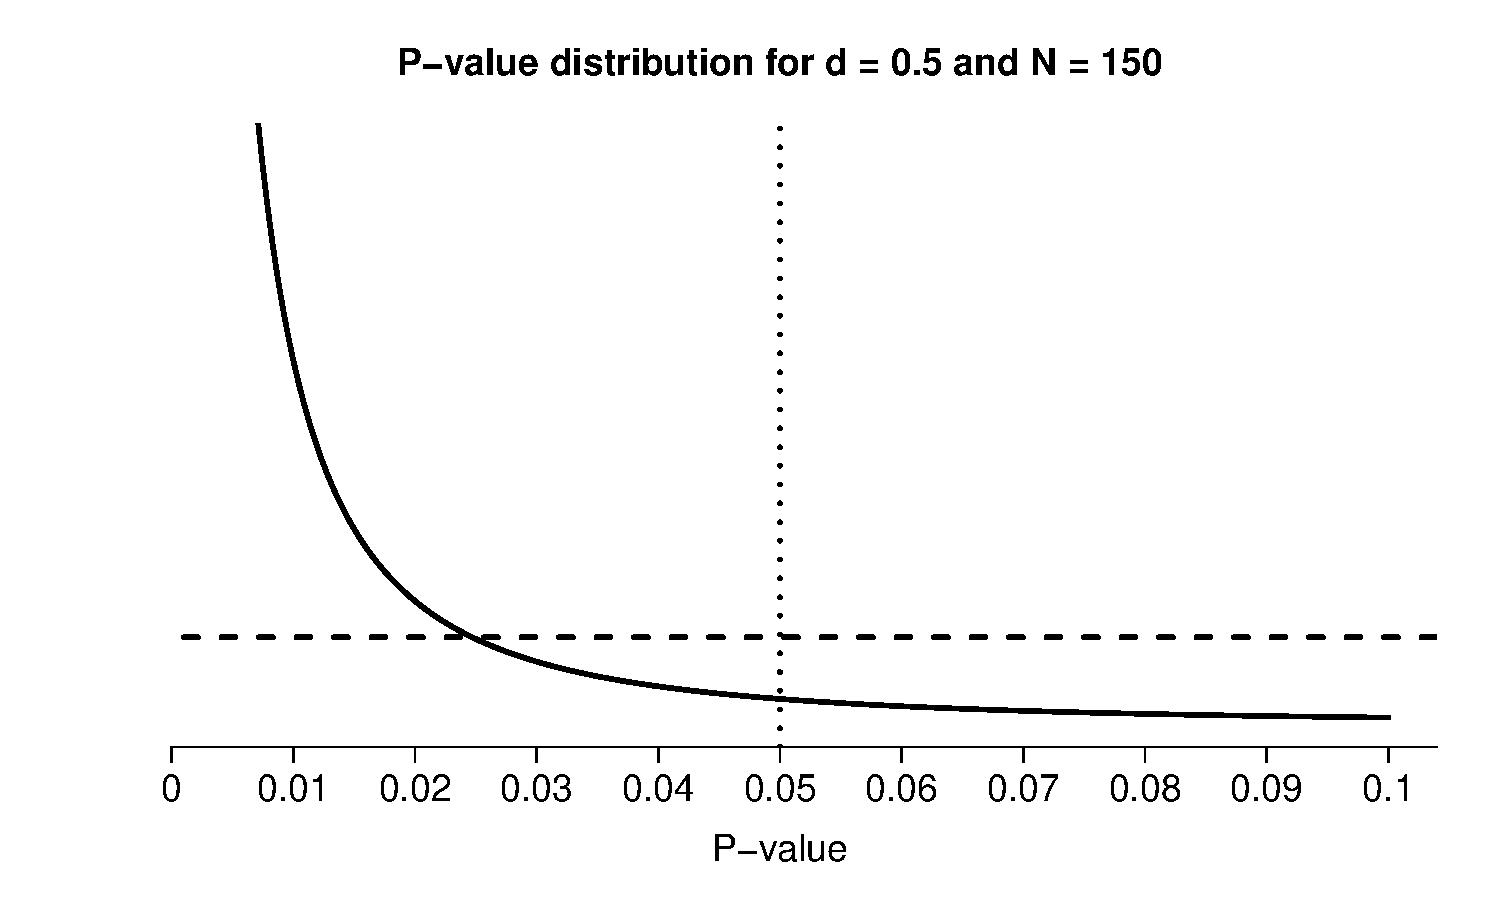
\includegraphics{Justify_in_Practice_files/figure-latex/p-plot-1.pdf}
\caption{\label{fig:p-plot}\emph{P}-value distributions for a two-sided independent \emph{t}-test with N = 150 and d = 0.5 (black curve) or d = 0 (horizontal dashed line) which illustrates how \emph{p}-values just below 0.05 can be more likely when there is no effect than when there is an effect.}
\end{figure}

Researchers often want to interpret a significant test result as `support' for the alternative hypothesis. In other words, in addition to controlling the \emph{error rate}, researchers might be interested in interpreting the \emph{relative evidence} in the data for null hypothesis over the alternative hypothesis. If so, it makes sense to choose the alpha level such that when a significant \emph{p}-value is observed, the \emph{p}-value is actually more likely when the alternative hypothesis is true than when the null hypothesis is true. This means that when statistical power is very high (e.g., the sample size is very large), the alpha level should be reduced. For example, if the alpha level in Figure \ref{fig:p-plot} is lowered to 0.02 then the alternative hypothesis is more likely than the null hypothesis for all significant \emph{p}-values that would be observed. This approach to justifying the alpha level can be seen as a frequentist/Bayesian compromise (Good, 1992). The error rate is controlled, but the alpha level is also set at a value that guarantees that whenever we reject the null hypothesis, the data is more likely under the alternative hypothesis, than under the null.

\hypertarget{minimizing-or-balancing-type-1-and-type-2-error-rates}{%
\subsection{Minimizing or Balancing Type 1 and Type 2 Error Rates}\label{minimizing-or-balancing-type-1-and-type-2-error-rates}}

If both Type 1 as Type 2 errors are costly, then it makes sense to optimally reduce both errors as you design studies. This leads to studies where you make decisions most efficiently. Researchers can choose to design a study with a statistical power and alpha level that minimizes the \emph{combined error rate}. For example, assuming H0 and H1 are a-priori equally probable (the prior probability for both is 0.5). With a Type 1 error rate of 0.05 and statistical power of 0.80 the combined error rate is (0.5×0.05 + 0.5×0.20) = 0.125. We could have chosen to set the alpha level in this study to 0.1. If the Type 1 error rate is 0.1, the statistical power (given the same sample size) would be 0.88, which means the combined error rate is (0.5×0.1 + 0.5×0.12) = 0.11. In other words, increasing the Type 1 error rate from 0.05 to 0.1 reduced the Type 1 error rate from 0.2 to 0.12, and the combined error rate from 0.125 to 0.11. In the latter scenario, our total probability of making an erroneous decision has become 0.015 smaller. As shown below, this approach can be extended to incorporate scenarios where the prior probability of H0 and H1 differ. Mudge, Baker, Edge, and Houlahan (2012) show that by choosing an alpha level based on the relative weight of Type 1 errors and Type 2 errors, and assuming beliefs about the prior probability that H0 and H1 are correct, decisions can be made more efficiently than when the default alpha level of 0.05 is used.

Winer (1962) writes: ``The frequent use of the .05 and .01 levels of significance is a matter of convention having little scientific or logical basis. When the power of tests is likely to be low under these levels of significance, and when Type 1 and Type 2 errors are of approximately equal importance, the .30 and .20 levels of significance may be more appropriate than the .05 and .01 levels.'' The reasoning here is that a design that has 70\% power for the smallest effect size of interest would not balance the Type 1 and Type 2 error rates in a sensible manner. Similarly, in huge datasets it might be possible to achieve very high levels of power for all effect sizes that are still considered meaningful. If such a study has 99\% power for effect sizes of interest, and thus a 1\% Type 2 error rate, but uses a 5\% alpha level, it also suffers from a lack of balance. This latter scenario is quite common in meta-analyses, where researchers by default use a 0.05 alpha level, while the meta-analysis typically have much higher power than 0.95 for all effect sizes of interest. In such cases, it seems sensible to lower the alpha level considerably.

Researchers can decide to either balance Type 1 and Type 2 error rates (e.g., setting both at 5\%), or minimize the combined error rate. For any given sample size and effect size of interest there is an alpha level that minimizes the combined error rates. Because the chosen alpha level also influences the statistical power, and the Type 2 error rate is therefore dependent upon the Type 1 error rate, minimizing or balancing error rates requires an iterative procedure.

As an example, imagine researchers plan to perform a study which will be analyzed with an independent two-sided \emph{t}-test. They plan to collect 50 participants per condition, and set their smallest effect size of interest to Cohen's d = 0.5. They think a Type 1 error is just as costly as a Type 2 error, and believe H0 is just as likely to be true as H1. The combined error rate is minimized when they set alpha to 0.13 (see Figure \ref{fig:weight-plot}, dotted line), which will give the study a Type 2 error rate of beta = 0.166 to detect effects of d = 0.5. The combined error rate is 0.148, while it would have been 0.177 if the alpha level was set at 5\%\footnote{For the same scenario, balanced error rates are alpha = 0.149 and beta = 0.149.}.

We see that increasing the alpha level reduced the combined error rate. The reduction in the combined error rate is not huge, but we have reduced the overall probability of making an error. More importantly, we have chosen an alpha level based on a justifiable principle, and clearly articulated the relative costs of a Type 1 and Type 2 error. Perhaps counter-intuitively, decision making is sometimes slightly more efficient after \emph{increasing} the alpha level from the default of 0.05. Had the sample size been much smaller, such as n = 10, the solid line in Figure \ref{fig:weight-plot} shows that the combined error rate will always be high, but it is minimized if we increase the alpha level to alpha to 0.283. If the sample size had been n = 100, the optimal alpha level to reduce the combined error rate (still assuming H0 and H1 have equal probabilities, and Type 1 and Type 2 errors are equally costly) is 0.0509 (the long-dashed line in Figure \ref{fig:weight-plot}).

\begin{figure}
\centering
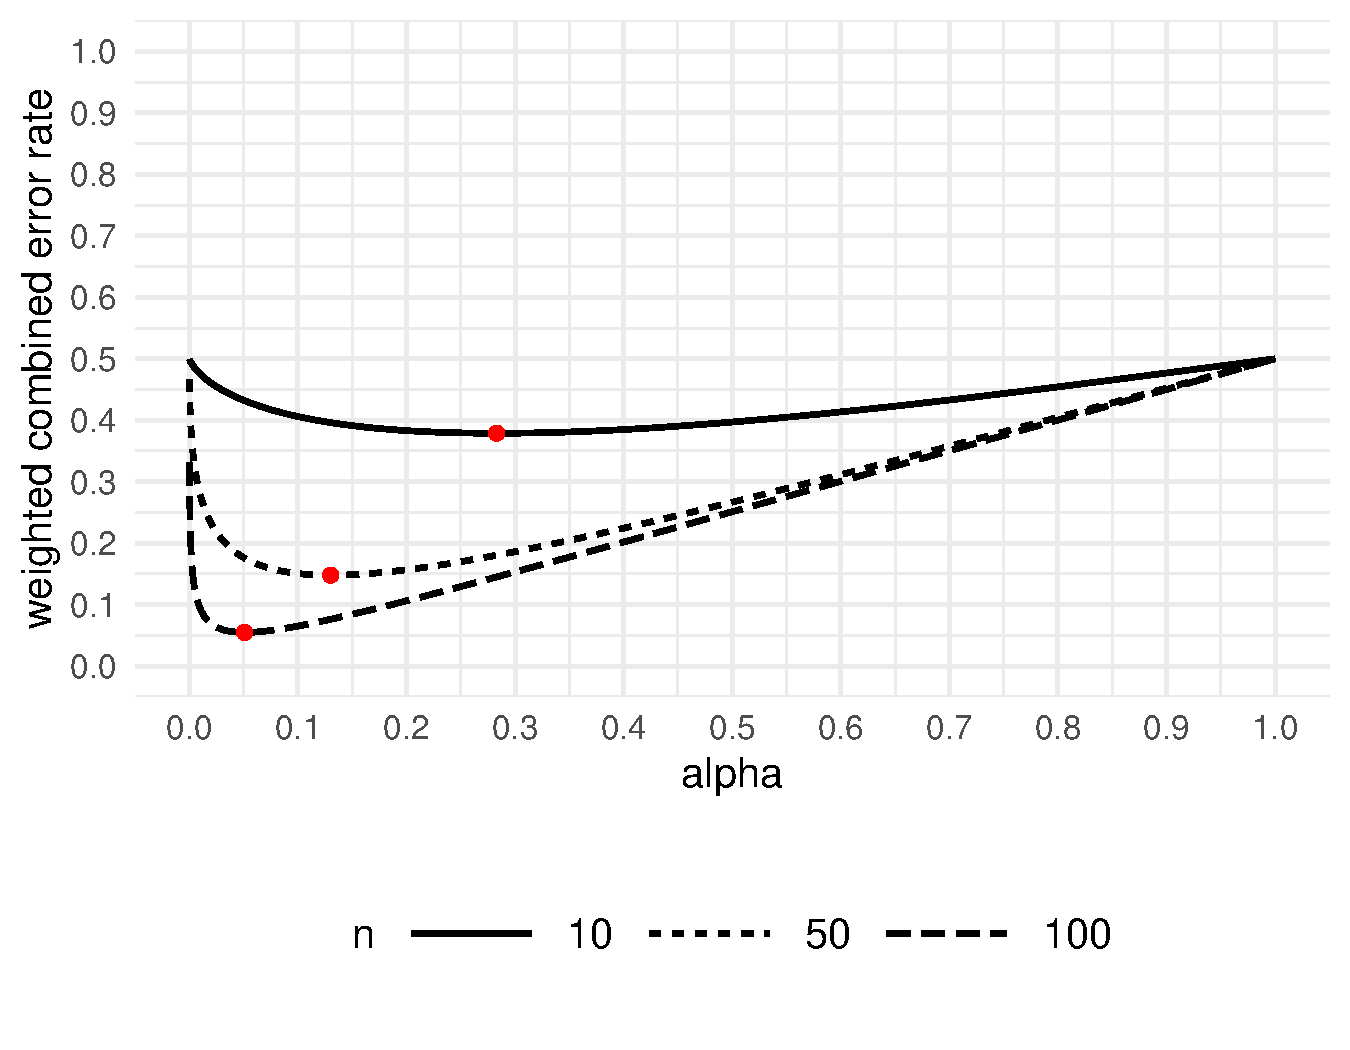
\includegraphics{Justify_in_Practice_files/figure-latex/weight-plot-1.pdf}
\caption{\label{fig:weight-plot}Weighted combined error rate (y-axis) for an independent \emph{t}-test with n = 10, n = 50, and n = 100 per group and a smallest effect of interest of d = 0.5, for all possible alpha levels (x-axis).}
\end{figure}

\hypertarget{weighing-the-relative-cost-of-errors}{%
\subsection{Weighing the Relative Cost of Errors}\label{weighing-the-relative-cost-of-errors}}

Cohen (1988) recommended a study design with a 5\% Type 1 error rate and a 20\% Type 2 error rate. The reason for this was that instead of weighing both types of errors equally, he felt ``Type I errors are of the order of four times as serious as Type II errors.'' The best weigh to determine the relative costs of Type 1 and Type 2 errors is by performing a cost-benefit analysis. As an example from another discipline, Field, Tyre, Jonzén, Rhodes, and Possingham (2004) quantify the relative costs of Type 1 errors when testing whether native species in Australia are declining. They find that when it comes to the Koala population, given its great economic value, a cost-benefit analysis indicates the alpha level should be set to 1. In other words, one should always act as if the population is declining, because the relative cost of a Type 2 error compared to a Type 1 error is practically infinite.

Although it can be difficult to formally quantify all factors that determine the costs of Type 1 and Type 2 errors, there is no reason to let the perfect be the enemy of the good. In research questions where there are no direct applications of the research findings, relative costs might be largely subjective, but it is still up to the researcher to determine an appropriate balance between Type 1 and Type 2 errors (Douglas, 2000). If you have a research strategy where you always follow up on an initial study testing a theoretical prediction with a replication and extension study, and want to innovate, you might want to weigh a Type 2 error more strongly than a Type 1 error. If you are relatively sure policies will be changed based on the outcome of your single study, or believe it will be unlikely that many researchers will have the resources to replicate your study, a Type 1 error rate might be weighed more strongly than a Type 2 error. There are no right or wrong answers, but you need to think through this question when you design a study.

If we adapt our calculations for the example above where researchers who plan to collect 50 participants per condition to detect a d = 0.5 effect, but now weigh the cost of Type 1 errors 4 times as much as Type 2 errors, balanced error rates are a Type 1 error rate of 0.0654 and a Type 2 error rate of 0.262. You will notice this is exactly the scenario Cohen describes, where a 5\% Type 1 error rate and 20\% Type 2 error rate is recommended, because he personally believed Type 1 errors should be considered 4 times as costly as Type 2 errors.

One could also aim to minimize error rates in the latter scenario by setting the Type 1 error rate to 0.0387 and the Type 2 error rate to 0.343. Remember the cost of a Type 1 error is four times as large as the cost of a Type 1 error. Imagine a Type 1 error has a cost of 400 and a Type 2 error has a cost of 100. We perform 100 studies, 50 where H0 is true and 50 where H1 is true. We will make 1.93 Type 1 errors and 17.14 Type 2 errors, with a respective cost of 773.6 and 1714, respectively. Figure \ref{fig:cost-plot} visualizes the weighted combined error rate for this study design across the all possible alpha levels. Compare this to the n = 50 line in Figure \ref{fig:weight-plot} to see the impact of the change in the weight of Type 1 compared to Type 2 errors.

\begin{figure}
\centering
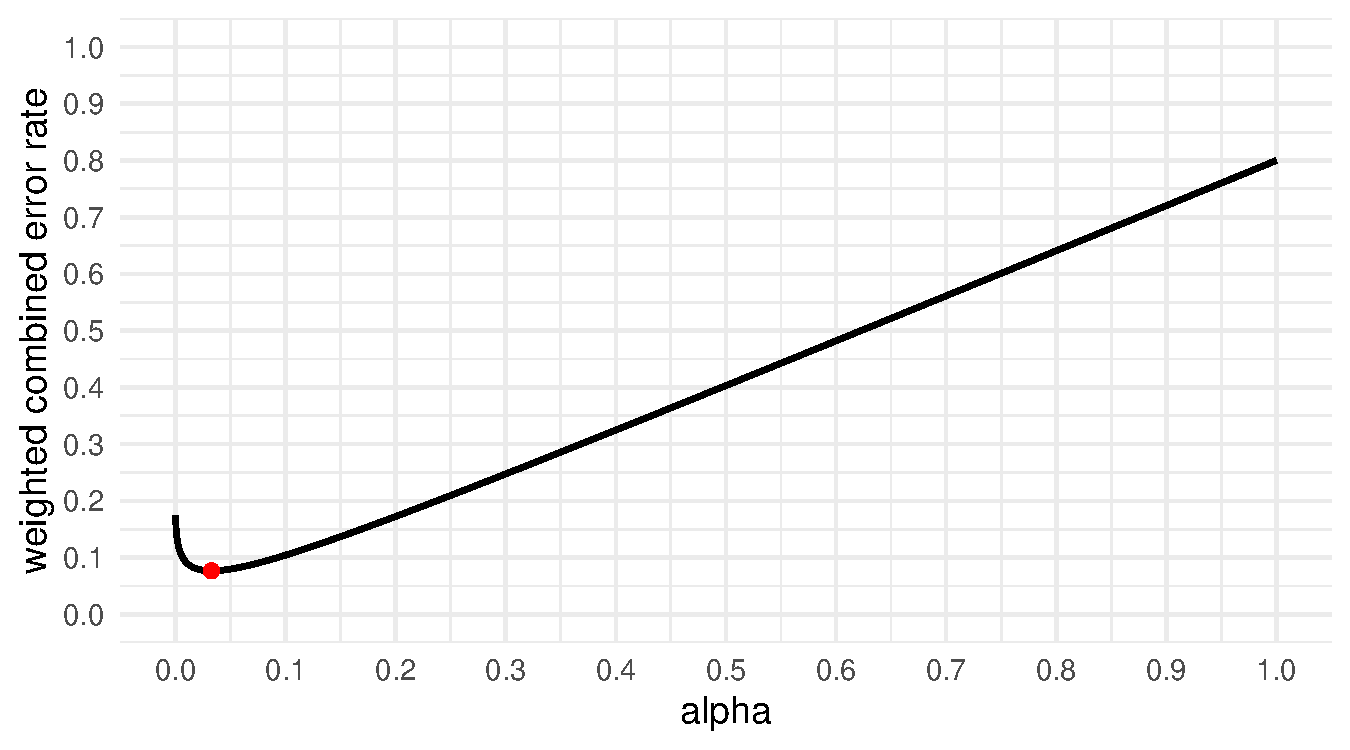
\includegraphics{Justify_in_Practice_files/figure-latex/cost-plot-1.pdf}
\caption{\label{fig:cost-plot}Weighted combined error rate (y-axis) for an independent \emph{t}-test with n = 50 per group and a smallest effect of interest of d = 0.5, where Type 1 errors are weighed 4 times as much as Type 2 errors, for all possible alpha levels (x-axis).}
\end{figure}

\hypertarget{incorporating-prior-probabilities}{%
\subsection{Incorporating prior probabilities}\label{incorporating-prior-probabilities}}

Miller and Ulrich (2019) explain how the choice for an optimal alpha level depends not just on the relative costs of Type 1 and Type 2 errors, but also on the base rate of true effects. In the extreme case, all studies a researcher designs test true hypotheses. In this case, there is no reason to worry about Type 1 errors, because a Type 1 error can only happen when the null hypothesis is true. Therefore, you can set the alpha level to 1 without any negative consequences. On the other hand, if the base rate of true hypotheses is very low, you are more likely to test a hypothesis where H0 is true, and the Type 1 error rate becomes an important consideration. For example, let's assume a researchers performs 1000 studies, and 100 studies test a hypothesis where H1 is true, and the remaining 900 studies test a hypothesis where H0 is true. With a 5\% Type 1 error rate and a 20\% Type 2 error rate this researcher will observe 900 × 0.05 = 45 Type 1 errors, and 100 × 0.2 = 20 Type 2 errors. Imagine Type 1 errors are weighed 4 times as much as Type 2 errors (hence our choice for a 5\% Type 1 error rate and a 20\% Type 2 error rate), so Type 1 errors cost 400 and Type 2 errors cost 100. Because of the fact the H0 is much more often true than H1, the expected cost of Type 1 errors is 45 × 400 = 18000, and the expected cost of Type 2 errors is 20 × 100 = 2000.

If H0 and H1 had been equally likely (both occur with 50\% probability) we should expect to make 500 × 0.05 = 25 Type 1 errors, and 500 × 0.2 = 100 Type 2 errors, and the expected cost of Type 1 errors is 25 × 400 = 10000, and the expected cost of Type 2 errors is 100 × 100 = 10000. Because the prior probabilities of H0 and H1 are not equal, the cost of Type 1 errors is not the same as the cost for Type 2 errors. If possible, researchers can take their expectations about the long run frequency of Type 1 and Type 2 errors into account, so that the expected costs of Type 1 and Type 2 errors are equal.

If you want to balance or minimize error rates in the long run, you should lower the alpha level as the prior probability of a null effect increases, or increase the alpha level as the prior probability of a true effect increases. Because the base rate of true hypotheses is unknown, this step requires a subjective judgment. This can not be avoided, because one always makes assumptions about base rates, even if the assumption is that a hypothesis is equally likely to be true as false (with both H1 and H0 having a 50\% probability). Assuming equal prior probabilities for H1 and H0, we saw above that balanced error rates assuming d = 0.5 and collection n = 50 per condition in a \emph{t}-test would imply a Type 1 error rate of 0.149 and a Type 2 error rate of 0.149. If you assume the null hypothesis is 10 times more likely than the alternative hypothesis (or the alternative hypothesis is 0.1 times as likely as the null hypothesis) then balanced error rates would require setting alpha to 0.0356 and the Type 2 error rate to 0.355. If you believe the alternative hypothesis is twice as likely to be true as the null hypothesis, balancing error rates in the long run would mean increasing the alpha level and increasing the power by choosing a Type 1 error rate of 0.213 and a Type 2 error rate of 0.107.

The two approaches (balancing error rates or minimizing error rates) typically yield quite similar results. Where minimizing error rates might be slightly more efficient, balancing error rates might be slightly more intuitive (especially when the prior probability of H0 and H1 is equal). Note that although there is always an optimal choice of the alpha level, there is always a range of values that yield quite similar weighted error rates. It is useful to plot weighted error rates as in Figure \ref{fig:cost-plot}. To balance or minimize error rates, researchers need to carefully consider the relative cost of Type 1 and Type 2 errors, the prior probability the null hypothesis is true, and the effect size they want to detect (Mudge, Baker, Edge, \& Houlahan, 2012), because these factors are used to calculate the weighted combined error rates \emph{w}:

\begin{equation}
\frac{(cost_{T1T2} \times \alpha + prior_{H1H0} \times \beta)}{prior_{H1H0}+cost_{T1T2}}
\label{eq:minimize}
\end{equation}

For example, imagine Type 1 errors are weighted 4 times as much as Type 2 errors (\(cost_{T1T2}\) = 4) and the alternative hypothesis is believed to be 2 times as likely as the null hypothesis (\(prior_{H1H0}\) = 10). With alpha = 0.213 and beta = 0.107 the weighted combined error rate is 0.142.

\hypertarget{sample-size-justification-when-minimizing-or-balancing-error-rates}{%
\subsection{Sample Size Justification when Minimizing or Balancing Error Rates}\label{sample-size-justification-when-minimizing-or-balancing-error-rates}}

So far we have illustrated how to perform what is known as a \emph{compromise power analysis} where the error rates are computed (in this case, the weighted combined error rate) as a function of the sample size, the effect size, and the desired ratio of Type 1 and Type 2 errors (Erdfelder, Faul, \& Buchner, 1996). However, in practice researchers will often want to justify their sample size based on an \emph{a-priori power analysis} where the required sample size is computed to achieve desired error rates, given an effect size of interest (Lakens, 2021). It is not possible to perform an a-priori power analysis where the combined error rates are minimized (this would just always recommend an infinitely large sample size), but it is possible to determine the sample size at which we achieve a certain desired weighted combined error rate. This requires researchers to specify the effect size of interest, and relative cost of Type 1 and Type 2 errors, the prior probabilities of H0 and H1, and the desired weighted combined error rate.

Imagine a researcher is interested in detecting an effect of Cohen's d = 0.5 with a two sample \emph{t}-test. The researcher believes Type 1 errors are equally costly as Type 2 errors, and believes a H0 is equally likely to be true as H1. They desire a weighted combined error rate of 5\%. We can optimize the weighted combined error rate as a function of the alpha level and sample size through an iterative procedure, that reveals a sample size of 105 participants in each independent group is required to achieve the desired weighted combined error rate. This sample size can also be computed directly with common power analysis software by entering the desired alpha level and statistical power directly. In this example, where Type 1 and Type 2 error rates are weighted equally, and the prior probability of H0 and H1 is assumed to be 0.5, the sample size is identical that required to achieve an alpha of 0.05 and a desired statistical power for d = 0.5 of 0.95. \textcolor{red}{[MAX, I think the figure is confusing - let's discuss. Also, the optimize function should go to n+1 (it now does not match gpower always, it can optimize the below the required error rate (e.g., 0.0491 but should go to the next sample size)). Also, the function does not seem to work if I change defaults (see code above)]}.

\begin{figure}
\centering
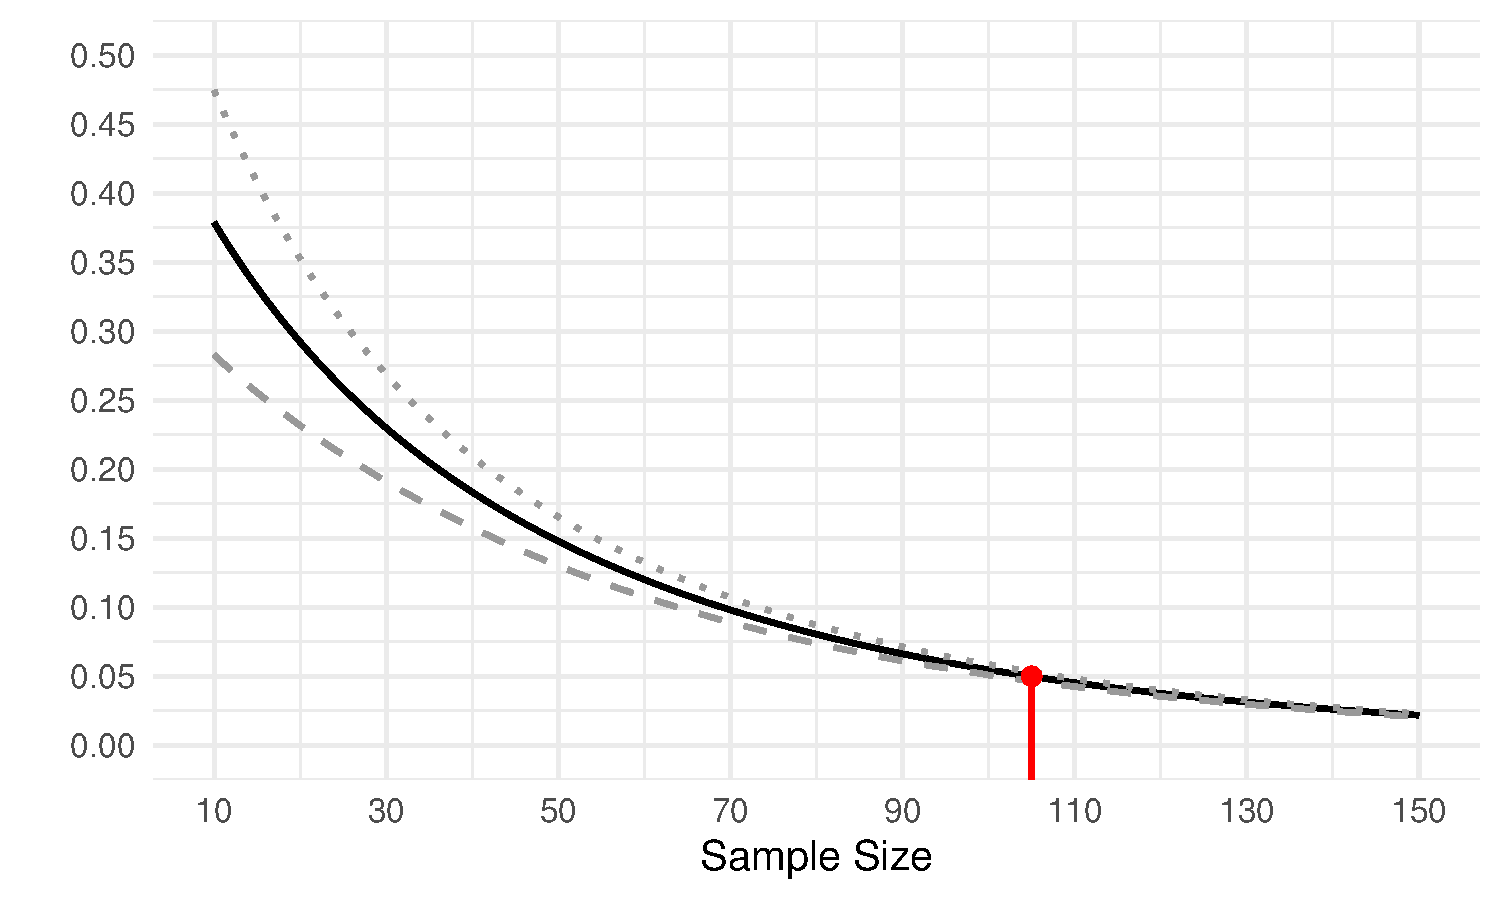
\includegraphics{Justify_in_Practice_files/figure-latex/error-plot-1.pdf}
\caption{\label{fig:error-plot}Weighted combined error rate (black), alpha (green), and beta (blue) for an independent \emph{t}-test as a function of sample size when the alpha level is justified to achieve lowest errors at each sample size.}
\end{figure}

\hypertarget{lowering-the-alpha-level-as-a-function-of-the-sample-size}{%
\subsection{Lowering the Alpha Level as a Function of the Sample Size}\label{lowering-the-alpha-level-as-a-function-of-the-sample-size}}

Formally controlling the costs of errors can be a challenge, as it requires researchers to specify relative costs of Type 1 and Type 2 errors, prior probabilities, and the effect size of interest. Due to this complexity, researchers might be tempted to fall back to the heuristic use of an alpha level of 0.05. Fisher (1971) referred to the default alpha level of 0.05 as a ``convenient convention,'' and it might suffice as a threshold to make scientific claims in a scientific system where we have limited resources and value independent replications (Tunç, Tunç, \& Lakens, 2021).

However, there is a well known limitation of using a fixed alpha level that has lead statisticians to recommend choosing an alph level as a function of the sample size. To understand the argument behind this recommendation, it is important to distinguish between statistical inferences based on error control and inferences based on likelihoods. An alpha level of 5\% will limit incorrect decisions to a desired maximum (in the long run, and when all test assumptions are met). However, from a likelihood perspective it is possible that the observed data is much more likely when the null hypothesis is true than when the alternative hypothesis is true, even when the observed \emph{p}-value is smaller than 0.05. This situation, known as Lindley's paradox, is visualized in Figure \ref{fig:p-plot}. It emerges because in frequentist statistics the critical value of a test approaches a limit as the sample size increases (e.g., \emph{t} = 1.96 for a two-sided \emph{t}-test with an alpha level of 0.05). In Bayesian statistics a critical value (e.g., a BF \textgreater{} 10) requires a larger test statistic as the sample size increases (see Jeffrey N. Rouder, Speckman, Sun, Morey, and Iverson (2009a) and Zellner (1971)).

To prevent situations where a frequentist rejects the null hypothesis based on p \textless{} 0.05, when the evidence in the test favors the null hypothesis over the alternative hypothesis (e.g., BF \textless{} 1) it is recommended to lower the alpha level as a function of the sample size. The need to do so is discussed extensively by Leamer (1978). He writes ``The rule of thumb quite popular now, that is, setting the significance level arbitrarily to .05, is shown to be deficient in the sense that from every reasonable viewpoint the significance level should be a decreasing function of sample size.'' This was already recognized by Harold Jeffreys (1939), who discusses ways to set the alpha level in the Neyman-Pearson approach to statistics: ``We should therefore get the best result, with any distribution of alpha, by some form that makes the ratio of the critical value to the standard error increase with n.~It appears then that whatever the distribution may be, the use of a fixed \emph{P} limit cannot be the one that will make the smallest number of mistakes.'' Similarly, Good (1992) notes: ``we have empirical evidence that sensible \emph{P} values are related to weights of evidence and, therefore, that \emph{P} values are not entirely without merit. The real objection to \emph{P} values is not that they usually are utter nonsense, but rather that they can be highly misleading, especially if the value of N is not also taken into account and is large.''

To prevent Lindley's paradox when using frequentist statistics one would need to adjust the alpha level in a way that the likelihood ratio (also called the Bayes factor) at the critical test statistic is not larger than 1. With such an alpha level, a significant \emph{p}-value will always be at least as likely if the alternative is true than if the null is true, which avoids Lindley's paradox. Faulkenberry (2019) and Jeffrey N. Rouder, Speckman, Sun, Morey, and Iverson (2009b) developed Bayes factors for \emph{t}-tests and ANOVAs which can calculate the Bayes factor from the test statistic and degrees of freedom. We developed a shiny app (link) that lowers the alpha level where necessary, such that the critical value that leads researchers to reject H0 is also high enough to guarantee that the data provide evidence in favor of H1.

There are two relatively arbitrary decisions that can be made about how to prevent Lindley's paradox, and Leamer (1978) and Good (1992) offer their own approaches. In our calculations we rely on a unit information prior.\footnote{For t-tests the shiny app also allows to use the more common Cauchy prior.} This prior is relatively wide which sometimes results in overstated evidence for H0, which means it is a conservative choice when attempting to prevent Lindley's paradox. This choice for an uninformative prior is itself a `convenient convention,' but researchers can lower the alpha level based on a more informed prior using the same logic by writing custom code. A benefit of the default use of the unit information prior is that, in contrast to previous approaches that aimed to calculate a Bayes factor for every \emph{p}-value (Colquhoun, 2017; e.g., D. Colquhoun, 2019) researchers do not need to specify the effect size under the alternative hypothesis. This lowers the barrier to adopting this approach in situations where it is difficult to specify a smallest effect size of interest or an expected effect size.

A second decision is the threshold of the Bayes factor used to lower the alpha level. Using a Bayes factor of 1 formally prevents Lindley's paradox, but this means it is in theory still possible to reject the null hypothesis when the data provide just as much evidence for H1 as for H0. Although it is important to note that researchers will often observe \emph{p}-values well below the critical value, and thus, in practice the evidence in the data will be substantially in favor of H1 when H0 is rejected, researchers might want to increase the threshold of the Bayes factor that is used to lower the alpha level to prevent weak evidence (H. Jeffreys, 1939) by setting the threshold to a larger value (e.g., BF \textgreater{} 3). Therefore, we extended the shiny app to allow researchers to adjust the alpha level in a way that a significant \emph{p}-value will always provide moderate or strong evidence against the null hypothesis.

We can illustrate the approach to lowering the alph level as a function of the sample size based on a study in Daryl Bem's infamous paper where he made the questionable claim that precognition is real (Bem, 2011). In study six of his paper, Bem reports the following one sample \emph{t}-tests \(t\)(149) = 1.80, \(p\) = .037, \(d\) = 0.15, \(p\) = .041 and \(t\)(149) = 1.77, \(p\) = .039, \(p\) = .041, as evidence for ``retroactive habituation.'' It seems like the \(p\)-values in this study are remarkably close to the 5\% threshold, especially given the sample size of 150 participants. Therefore, let us consider which alpha level Bem would have needed to use to avoid Lindley's Paradox, and to achieve moderate or strong evidence.

To avoid Lindley's paradox, Bem would need to use an alpha level of 0.0274. In other words, the observed \emph{p}-value is more likely under the null hypothesis than under the alternative. However, it seems desirable to require at least moderate evidence for the alternative before claiming a discovery. To achieve this Bem would have needed to use a alpha level of 0.0077. To provide strong evidence given a significant \emph{p}-value, he would have needed to use an even lower alpha level of 0.0020. We can see from this example, that \emph{p} = 0.05 is too low of an evidential standard under large sample sizes.

For small sample sizes it is possible to guarantee that a significant result is evidence for the alternative hypothesis using a higher alpha level than 0.05. For example, for an independent \emph{t}-test this is achieved whenever the sample size is smaller than 84 based on a Bayes factor threshold of 1. It is not recommended to use this procedure to increase the sample size above a conventional choice of an alpha level (e.g., 0.05). This approach to the justification of an alpha level assumes researchers foremost want to control the error rat, and secondary prefer to prevent Lindley's paradox by reducing the alpha level as a function of the sample size where needed.

\hypertarget{comparison-of-the-two-approaches}{%
\subsection{Comparison of The Two Approaches}\label{comparison-of-the-two-approaches}}

When should we minimize or balance error rates and when should we avoid Lindley's paradox? In practice, it might be most convenient to use the first approach whenever there is enough information to conduct a power analysis, and if researchers do not feel they can specify a smallest effect size of interest, to fall back on the second approach. Alternatively, one can also apply both approaches and choose the one that is more conservative (i.e., results in a lower alpha level). In addition, researchers aiming to find a compromise between frequentist and Bayesian inference might be drawn more strongly towards the second approach Good (1992).

Figure \ref{fig:heatmap} shows which alpha level is larger as a function of sample size (per group) and expected effect size for a two-sample \emph{t}-test. For green values minimizing error rates resulted in higher alpha values, whereas red areas mean that avoiding the Lindley paradox resulted in higher alpha levels. We can see that when the expected effect size increases (x-axis) the alpha level will be smaller when using the method that minimizes error rates. This is mostly a result of how we set up the likelihood ratio calculations. Due to the unit information prior the method trying to avoid the Lindley paradox is not sensitive to the expected effect size. If the sample size increases on the other hand (y-axis) the alpha level reduces faster when avoiding the Lindley paradox then when minimizing error rates.

\textcolor{red}{[MAX, this is an insightful plot, but, it makes more sense to show the alpha levels (say, a contour plot with lines for alpha 0.01, 0.02, 0.03, 0.04, 0.05). Also, we do not really require them to choose between these 2. I guess the 2 approaches really are fundamentally different philosophies - so the choice is not dependent on the alpha anyway?]}.

\begin{figure}
\centering
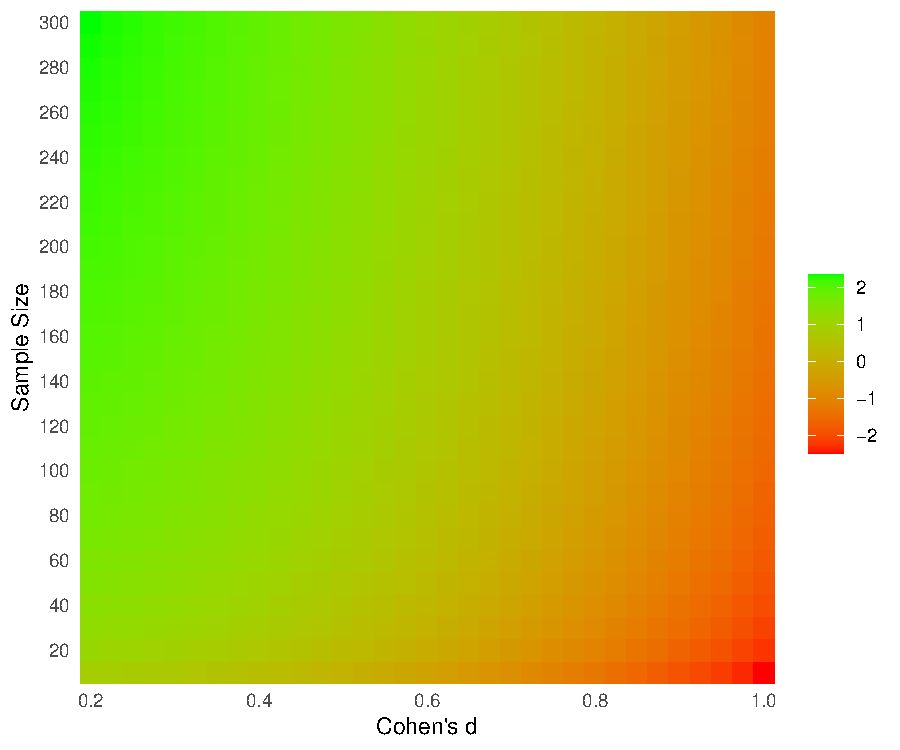
\includegraphics{Justify_in_Practice_files/figure-latex/heatmap-1.pdf}
\caption{\label{fig:heatmap}Heatmap of log(alpha\_minimize/alpha\_lindley) as a function of sample size and expected effect size.}
\end{figure}

\hypertarget{discussion}{%
\section{Discussion}\label{discussion}}

Editors and reviewers should \emph{always} ask authors to justify their choice of error rates, whenever researchers use data to make decisions about the presence or absence of an effect. As Skipper, Guenther, and Nass (1967) remarks: ``If, in contrast with present policy, it were conventional that editorial readers for professional journals routinely asked:''What justification is there for this level of significance? authors might be less likely to indiscriminately select an alpha level from the field of popular eligibles." In a Neyman-Pearson approach to statistics, the alpha level should be set before the data is collected. When reviewers of for example a Registered Report would ask authors to justify their alpha level, it would be convenient if they can recommend some approaches to do so. The current manuscript hopefully helps to fill this gap.

If a power analysis can be performed (i.e., whenever a desired or expected effect size of interest can be specified) and relative costs and priors can be specified, researchers can design efficient by minimizing or balancing error rates, optimizing informational value, or aiming for specific posterior probabilities. If it is difficult to specify these aspects of the study, researchers can fall back to the approach where the alpha level is reduced as a function of the sample size.

A Shiny app is available that allows users to perform the calculations recommended in this article. It can be used to minimize or balance alpha and beta, which works by specifying the effect size of interest and the sample size, as well as an analytic power calculation. The effect size should be determined as in a normal a-priori power analysis (preferably based on the smallest effect size of interest, for recommendations, see Albers and Lakens (2018)). Alternatively, researchers lower the alpha level as a function of the sample size by specifying only their sample size. Whichever approach is used, it is strongly recommended to preregister the alpha level that researchers plan to use before the data is collected.

Because of the strong overreliance on a 5\% error rate when designing studies, we have seen relatively few people attempt to justify their alpha level. As researchers start to justify their alpha, we will hopefully see the development of good examples and best practices for psychological science. It might be a challenge to get started, but the two approaches presented in the current article are one way to move away from the mindless use of a 5\% alpha level. There is a lot to gain, and justifying alpha levels should improve our statistical inferences and increase the efficiency of the research we perform.

\hypertarget{references}{%
\section{References}\label{references}}

\begingroup

\interlinepenalty = 10000

\hypertarget{refs}{}
\begin{CSLReferences}{1}{0}
\leavevmode\hypertarget{ref-albers_when_2018}{}%
Albers, C., \& Lakens, D. (2018). When power analyses based on pilot data are biased: {Inaccurate} effect size estimators and follow-up bias. \emph{Journal of Experimental Social Psychology}, \emph{74}, 187--195. \url{https://doi.org/10.1016/j.jesp.2017.09.004}

\leavevmode\hypertarget{ref-bakan_test_1966}{}%
Bakan, D. (1966). The test of significance in psychological research. \emph{Psychological Bulletin}, \emph{66}(6), 423--437.

\leavevmode\hypertarget{ref-bem2011feeling}{}%
Bem, D. J. (2011). Feeling the future: Experimental evidence for anomalous retroactive influences on cognition and affect. \emph{Journal of Personality and Social Psychology}, \emph{100}(3), 407.

\leavevmode\hypertarget{ref-cohen_statistical_1988}{}%
Cohen, J. (1988). \emph{Statistical power analysis for the behavioral sciences} (2nd ed). {Hillsdale, N.J}: {L. Erlbaum Associates}.

\leavevmode\hypertarget{ref-colquhoun2017reproducibility}{}%
Colquhoun. (2017). The reproducibility of research and the misinterpretation of p-values. \emph{Royal Society Open Science}, \emph{4}(12), 171085.

\leavevmode\hypertarget{ref-colquhoun2019false}{}%
Colquhoun, D. (2019). The false positive risk: A proposal concerning what to do about p-values. \emph{The American Statistician}, \emph{73}(sup1), 192--201.

\leavevmode\hypertarget{ref-cousins_jeffreyslindley_2017}{}%
Cousins, R. D. (2017). The {Jeffreys}{{Lindley}} paradox and discovery criteria in high energy physics. \emph{Synthese}, \emph{194}(2), 395--432. \url{https://doi.org/10.1007/s11229-014-0525-z}

\leavevmode\hypertarget{ref-cowles_origins_1982}{}%
Cowles, M., \& Davis, C. (1982). On the origins of the. 05 level of statistical significance. \emph{American Psychologist}, \emph{37}(5), 553.

\leavevmode\hypertarget{ref-cumming_replication_2008}{}%
Cumming, G. (2008). Replication and {\emph{p}} {Intervals}: {\emph{P}} {Values Predict} the {Future Only Vaguely}, but {Confidence Intervals Do Much Better}. \emph{Perspectives on Psychological Science}, \emph{3}(4), 286--300. \url{https://doi.org/10.1111/j.1745-6924.2008.00079.x}

\leavevmode\hypertarget{ref-douglas_inductive_2000}{}%
Douglas, H. E. (2000). Inductive risk and values in science. \emph{Philosophy of Science}, \emph{67}(4), 559--579.

\leavevmode\hypertarget{ref-erdfelder_gpower_1996}{}%
Erdfelder, E., Faul, F., \& Buchner, A. (1996). {GPOWER}: {A} general power analysis program. \emph{Behavior Research Methods, Instruments, \& Computers}, \emph{28}(1), 1--11. \url{https://doi.org/10.3758/BF03203630}

\leavevmode\hypertarget{ref-faulkenberry2019estimating}{}%
Faulkenberry, T. J. (2019). Estimating evidential value from analysis of variance summaries: A comment on ly et al.(2018). \emph{Advances in Methods and Practices in Psychological Science}, \emph{2}(4), 406--409.

\leavevmode\hypertarget{ref-field_minimizing_2004}{}%
Field, S. A., Tyre, A. J., Jonzén, N., Rhodes, J. R., \& Possingham, H. P. (2004). Minimizing the cost of environmental management decisions by optimizing statistical thresholds. \emph{Ecology Letters}, \emph{7}(8), 669--675.

\leavevmode\hypertarget{ref-fisher_design_1935}{}%
Fisher, Ronald Aylmer. (1935). \emph{The design of experiments}. {Oliver And Boyd; Edinburgh; London}.

\leavevmode\hypertarget{ref-fisher_design_1971}{}%
Fisher, Ronald A. (1971). \emph{The {Design} of {Experiments}} (9 edition). New York: Macmillan Pub Co.

\leavevmode\hypertarget{ref-gigerenzer_statistical_2018}{}%
Gigerenzer, G. (2018). Statistical {Rituals}: {The Replication Delusion} and {How We Got There}. \emph{Advances in Methods and Practices in Psychological Science}, 2515245918771329. \url{https://doi.org/10.1177/2515245918771329}

\leavevmode\hypertarget{ref-good_bayes-non-bayes_1992}{}%
Good, I. J. (1992). The {Bayes}-{Non}-{Bayes Compromise}: {A Brief Review}. \emph{Journal of the American Statistical Association}, \emph{87}(419), 597. \url{https://doi.org/10.2307/2290192}

\leavevmode\hypertarget{ref-jeffreys_theory_1939}{}%
Jeffreys, Harold. (1939). \emph{Theory of probability} (1st ed). {Oxford {[}Oxfordshire{]} : New York}: {Clarendon Press ; Oxford University Press}.

\leavevmode\hypertarget{ref-Jeffreys1939}{}%
Jeffreys, H. (1939). \emph{Theory of probability} (1st ed.). Oxford, UK: Oxford University Press.

\leavevmode\hypertarget{ref-kennedy-shaffer_before_2019}{}%
Kennedy-Shaffer, L. (2019). Before p {\(<\)} 0.05 to {Beyond} p {\(<\)} 0.05: {Using History} to {Contextualize} p-{Values} and {Significance Testing}. \emph{The American Statistician}, \emph{73}(sup1), 82--90. \url{https://doi.org/10.1080/00031305.2018.1537891}

\leavevmode\hypertarget{ref-lakens_sample_2021}{}%
Lakens, D. (2021). \emph{Sample {Size} {Justification}}. PsyArXiv. \url{https://doi.org/10.31234/osf.io/9d3yf}

\leavevmode\hypertarget{ref-leamer_specification_1978}{}%
Leamer, E. E. (1978). \emph{Specification {Searches}: {Ad Hoc Inference} with {Nonexperimental Data}} (1 edition). {New York usw.}: {Wiley}.

\leavevmode\hypertarget{ref-lindley_statistical_1957}{}%
Lindley, D. V. (1957). A statistical paradox. \emph{Biometrika}, \emph{44}(1/2), 187--192.

\leavevmode\hypertarget{ref-miller_quest_2019}{}%
Miller, J., \& Ulrich, R. (2019). The quest for an optimal alpha. \emph{PLOS ONE}, \emph{14}(1), e0208631. \url{https://doi.org/10.1371/journal.pone.0208631}

\leavevmode\hypertarget{ref-mudge_setting_2012}{}%
Mudge, J. F., Baker, L. F., Edge, C. B., \& Houlahan, J. E. (2012). Setting an {Optimal} {\(\alpha\)} {That Minimizes Errors} in {Null Hypothesis Significance Tests}. \emph{PLOS ONE}, \emph{7}(2), e32734. \url{https://doi.org/10.1371/journal.pone.0032734}

\leavevmode\hypertarget{ref-neyman_problem_1933}{}%
Neyman, J., \& Pearson, E. S. (1933). On the {Problem} of the {Most Efficient Tests} of {Statistical Hypotheses}. \emph{Philosophical Transactions of the Royal Society of London A: Mathematical, Physical and Engineering Sciences}, \emph{231}(694-706), 289--337. \url{https://doi.org/10.1098/rsta.1933.0009}

\leavevmode\hypertarget{ref-rouder_bayesian_2009}{}%
Rouder, Jeffrey N., Speckman, P. L., Sun, D., Morey, R. D., \& Iverson, G. (2009a). Bayesian t tests for accepting and rejecting the null hypothesis. \emph{Psychonomic Bulletin \& Review}, \emph{16}(2), 225--237. \url{https://doi.org/10.3758/PBR.16.2.225}

\leavevmode\hypertarget{ref-rouder2009bayesian}{}%
Rouder, Jeffrey N., Speckman, P. L., Sun, D., Morey, R. D., \& Iverson, G. (2009b). Bayesian t tests for accepting and rejecting the null hypothesis. \emph{Psychonomic Bulletin \& Review}, \emph{16}(2), 225--237.

\leavevmode\hypertarget{ref-skipper_sacredness_1967}{}%
Skipper, J. K., Guenther, A. L., \& Nass, G. (1967). The {Sacredness} of .05: {A Note} concerning the {Uses} of {Statistical Levels} of {Significance} in {Social Science}. \emph{The American Sociologist}, \emph{2}(1), 16--18.

\leavevmode\hypertarget{ref-tunc_epistemic_2021}{}%
Tunç, D. U., Tunç, M. N., \& Lakens, D. (2021). \emph{The {Epistemic} and {Pragmatic} {Function} of {Dichotomous} {Claims} {Based} on {Statistical} {Hypothesis} {Tests}}. PsyArXiv. \url{https://doi.org/10.31234/osf.io/af9by}

\leavevmode\hypertarget{ref-winer_statistical_1962}{}%
Winer, B. J. (1962). \emph{Statistical principles in experimental design}. {New York : McGraw-Hill}.

\leavevmode\hypertarget{ref-zellner_introduction_1971}{}%
Zellner, A. (1971). \emph{An introduction to {Bayesian} inference in econometrics}. {New York}: {Wiley}.

\end{CSLReferences}

\endgroup


\end{document}
